\documentclass{article}
\usepackage[utf8]{inputenc}
\usepackage{amsmath}
\usepackage{longtable}
\usepackage{lscape}

\title{Lallemand Yeast Analysis}
\author{Peeter Meos \\ Liubov Kyaes \\ Tanel Peet \\Ott Keki{\v s}ev}
\date{March 2019}

\begin{document}

\maketitle

\tableofcontents

\section{Introduction}
Quick brown fox...
\subsection{Process Description}
Process description for yeast fermentation goes here with all the steps F1-F8.

\section{Data Preparation}
The time series data describing the process arrived in a form of CSV files. The automation system providing the data had split the data vertically into a number of separate files. That is the variables describing the data are grouped into separate files, with one file consisting the entire length of time series (March - December 2018). The process steps were as follows: F2, F4, F5, F6, F7, F8. Additionally we were given data on three processes: CSep, MO and SP. The automation system collects the data at 10 minute interval, but in the time stamps themselves between the respective CSV files vary within that interval. That is, even though all CSV files for a given process step have the same number of rows, the timestaps for these rows are shifted but remain inside 10 minute window. Therefore we rounded all timestamps to the nearest smaller 10 minute point. That allowed the time stamps to match and data to be merged.

\subsection{Cycle Identification}
The F-process data were time stamped and also enriched with process time field. Therefore it was easy for these process steps to mark the cycles. When the field \texttt{step\_time} was zero, the production line was considered idle. The value change from zero to non-zero was considered as a marker for start of production cycle. Counting cumulatively the number of start markers allowed us to give a sequence number for each production cycle in each F-production step.

\subsection{Labelling}
As extra data we were given labels for 12 production cycles. The labels were titled ''reject'', ''restrict'' and ''release''. In order to know which cycles to label were additionally given production records in a form of PDF files with handwritten notes. A production record contained dates for process steps of F2 and following F4 or F5. We matched manually those dates with our labelling described above. We assumed that the dates in the PDF files marked the \emph{beginning} of the production step. However, in two cases of F2 we were not able to establish that match and picked the \emph{preceding} cycle label in the data. The rationale for that the date was recorded during the cycle and the production itself had started the previous day. This proved again, that manual data recording is inherently inconsistent and error prone. Therefore, one of our recommendations of our short analysis is to preferably automate the process. If the full automation is not possible, the HMI should be developed that ensures the consistency of timestamps in the recorded data. The full set of recommendations are described in more detail in the last section of this report. The cycle numbers in the data with the respective labels are displayed in the table below.

%\begin{tabular}
% Insert the cycle numbers here
%\end{tabular}

\section{Exploratory Data Analysis}
Initally for EDA we concentrated to process steps F2 and F4 since majority of the labelled data was situated there. After completing those we also took a look at F5 and the remaining data sets. The data itself is of acceptable quality with no additional changes necessary. The time series inside a given process step contained, however, various levels of information. Some series were almost exclusively either zero, static, or missing. Since these series do not have at least within this study any explanatory power, we cut these series out. The table below displays the time series that were left to describe each process.

Insert F2 series here
Describe the length of cycle in \texttt{step\_time}

Insert F4 series here
Describe \texttt{step\_time}

Insert F5 series here.
Describe \texttt{step\_time}

\section{Model Development}
\begin{align}
    min \sum_{i \in I}{X_i}    
\end{align}

\section{Feature Engineering}
Analysis of variables based on step times to identify some interruption in data recordings or process.  (parameters collection and representation based on step time and timestamps)

Study of variables. Using multivariate Principal Component Analysis (PCA) method for reducing dimensionality. The method determines the number of principal components and help to identify outliers. The original dataset had a plenty correlated and uncorrelated variables and dimensionality reduction can be a very useful step for visualizing and processing high-dimensional datasets.  PCA was used for data understanding as it allowing most of the variability to be explained using fewer variables.

 PCA was performed in few steps: determining the number of principal components, interpreting each principal component in terms of the original variables and identifying outliers. So, the first step of exploratory analysis was performing preliminary feature selection operations in order to bring the number of variables to a manageable range.
 
 F2, F4, F5 Data Classification.  For prediction a status the Linear Discriminant Analysis (LDA) was applied on PCA-’transformed’ data afterwards. The expectation was, that performing PCA before LDA model should give a little better result. LDA explicitly attempts to model the difference between the classes of data and is used when groups are known a priori.  LDA was run on labelled samples and then applied to unlabeled F2, F4 and F5 data.
 
 Analysis of variables to find out deviations from mean values between status groups. Boxplotting.  Applied on classified dataset (predicted labels/statuses) 

NB. Tools > All data analysis was done in R. PCA was performed using the built-in R functions prcomp(), princomp() and R package factoextra to create the visualization. For LDA there was used R package MASS. 



% Conclusions section
\section{Conclusions}
\label{sec:conclusions}
During exploration and preparation of the given datasets the following was noticed:

\paragraph{Overall quality was acceptable} There were some N/A variables with null values or missing measurements. The variables nature (data types) vary: process duration measures of step times, constant values of temperature, air and other conditions, boolean values, etc. However, the structure of variables is not homogeneous. Mainly variables represent a specified volume or mass of ingredients from manufacturing formulas, however, the data also consist of process condition measurements, such as an air or water temperatures.
    
\paragraph{Quantities} Provided \emph{sample data} with labels/status information (eg. the quantities of products that were released and rejected) \emph{is not sufficient enough for research}. 
    
\paragraph{Manual data} Furthermore, information about \emph{seed/batch number and statuses were matched manually} and therefore significant \emph{a probability of error} may exist – not all observations may have correct references to the yeast production \emph{cycle start and end times}.
    
\paragraph{Timestamps} In some cases, Date and Time data integrity is loosely presented and the assurance that the data is correctly merged is not consistent.
    
\paragraph{Classification} Even though the prediction of the status within given parameters was not very reliable, it was still possible. In the future, with improved input data (better matching and more class samples), the prediction precision could be increased.

\paragraph{Analysis conclusions} From the data analysis the following can be concluded:
\begin{itemize}
    \item The dataset is currently too small and unbalanced to produce statistically significant and reliable results. Moreover, the dataset is not sufficient yet to build reliable machine learning models.
    \item The variance between the process data of ``rejected'' and ``released'' batches appears to be significant in process step F2 and substantiates further research, whether these difference can influence the mutations and the quality of the yeast.
    \item In steps F4 and F5 the data is inconclusive and at current state is not able to provide any interesting insight. We recommend to collect more data, see Recommendations section of this paper.
\end{itemize}

% Recommendations section
\section{Recommendations}
Having completed the initial analysis of the yeast production process we have the following recommendations for further process improvements and better analytical insight:

\begin{itemize}
\item Digitize and automate if possible the current manual data collection on the production batches that is at present time in a form of scanned PDF files. The current system is error prone and does not lend itself easily for analytics.
\item Consider automatic loading of process data that is currently in CSV files into a time series database. That will provide for long term data storage and ease the preparatory steps for any future analytics on the fermentation process.
\end{itemize}

\subsection{Data Collection}
\paragraph{Labelling of parametric data with quality control information.}
Currently the classification and labelling of production batches is done manually, by guessing the batch production start and end times and labelling the recorded data accordingly. Therefore, the quality of labelling is a potential source of inaccuracies. The question of \emph{which measurements correspond to ‘Rejected’ and which ones correspond to ’Released’ statuses and  which measurements belongs to ‘Seed’ number 4151 and which ones to ‘Seed’ number 5292?} should be answered automatically.

\paragraph{Glossary} For further analysis and data storage create data glossary that describes all variables and terms used. This will limit possible future confusions in interpreting the data. Such glossary and metadata is an important portion of organizational data governance and data management.

Additionally, in order to analyze the parameters collected from the yeast cultivation process online (and offline) and identifying the deviations that cause quality problems, it is required to have enough historical data that allows to capture information about exact batch numbers and statuses with regards to time and production cycle. 

\paragraph{Automation of currently manual data collection.}
Recommend to automate collection of status information such as:
\begin{itemize}
    \item Production Date (MM-DD-YYYY)
    \item Strain
    \item Seed batch number
    \item Commercial batch number
    \item Lot no
    \item Status - quality control decision: Rejected, Released, Restricted release
\end{itemize}

Currently the relationship between time series data from separate production steps is merged and matched manually (eg. linking steps F2 and F4). That linkage should be automated.

\paragraph{Grouping parametric data into production batches.}
Every time\-stamped row of parametric data should be grouped into a respective production batch. As many observations belong to the one production batch (M:1) that means approx. 3 days duration for the one particular seed/batch, so after matching the data it should not have \emph{gaps or overlaps} in time period.  

Proposed new records to process parametric time series data on production batches: 
\begin{itemize}
    \item production line active / not active
    \item new batch start point / no change
    \item batch standing / running (batch serial number has to be assigned) 
\end{itemize}

\paragraph{Paperless Data Collection Consideration.}
\begin{itemize}
    \item Data provided on fermentation sheets (ie "7442ferm sheets"), contains manually measured values of the pH, spin test and other necessary variables. However they are \emph{not currently sufficient for analysis} and it is required to \emph{collect such historical data in digital and preferably automated manner}. 
    \item Making some fields ‘mandatory’ helps to submit data without missing it and therefore increase \emph{data completeness} (whether there are any gaps in the data from what was expected to be collected, and what was actually collected).
    \item Make sure that \emph{data integrity} is enforced. That is, that the data has not been changed when performing any operation on them, whether it is transfer, storage, display or during data preparation.
\end{itemize}

\subsection{Data Preparation}
To improve data preparation historical data instead of CSV files could be stored in some database tables or at least \emph{previously merged files corresponding to original time stamp and business process step}.

The main idea here is to have  precise mapping of date and time along the whole process to be able to monitor 1 batch from start to end like a holistic process work flow (for example to merge events from F1 $\,\to\,$ F2 $\,\to\,$ F4 steps vertically or horizontally, following and keeping  the full production time interval (approx. 3 days) required for producing the one yeast seed /batch.) 

Yeast separation, storage container data could be also referred to batch, seed and production dates. 

\subsection{Data Analysis}
We propose the following improvements for future data analyses:

\paragraph{Additional data collection.} Having more samples with labelled observations (Strain, Seed, Status) give higher probability to identify deviations that cause quality problem, identify which variables measurements impact quality and predict the production result /status.
\paragraph{Digitize manual data.} Having paperless recorded variables (i.e. pH) included to modelling to allow for more holistic analysis and modelling of the collected parameters. 


\listoffigures

\appendix
% Data description table goes to annex
\begin{landscape}
\section{Data Description}
\begin{center}
\begin{longtable}{l | p{5cm} | p{1.5cm} | p{10cm}}
\label{tab:data}
No & Data Source &	Data Origin	& Description \\
\hline
1 &	F1 data, 2 csv files	& provided & \\
2 &	F2 data,  5 csv files	& provided &	49092 rows, 0-211 cycles, 44 var, Initial fermentation data \\
3 & F4 data, 7 csv files	& provided &	49092 rows, 0-213 cycles, 60 var, yeast product data \\
4 &	F5 data, 6 csv files	& provided &	49093 rows, 0-282 cycles, 52 var, Commercial yeast product data \\
5 &	F7 data, 6 csv files	& provided &	49092 rows, 0-225 cycles, 52 variables \\
6 &	F8 data, 6 csv files	& provided &	49092 rows, 0-135 cycles, 52 variables\\
7 & CSep data, 3 csv files	&provided \\	
8 &	MO data, 17 csv files	&provided \\	
9 &	Seps data, 9 csv files	&provided \\	
10&	SR data, 11 csv files	&provided \\
11&	Manual fermentation recordings,  
F2-F4 10 pdf, F5 2 pdf files&	provided&	processes manually filled in pdf. Data contains only F4 and F5 fermentations recordings  \\
12&	Brown colonies ferms, word doc
(Quality control results for few F4 and F5 batches)	&provided&	Data has attributes
\begin{itemize}
    \item Production Date (MM-DD-YYYY) -finished product date
    \item Strain (yeast strain no 7442 only)
    \item Seed - batch number
    \item Commercial – if F5
    \item Lot no - number of batches
    \item 	Status - quality control decision: Rejected, Released, Restricted release)
\end{itemize} \\
13&	Data Parameters - Excel with fermentation variable details  	&provided&Glossary, some variables description. Mainly variables represent a specified volume or mass of ingredients from yeast manufacturing formulas, also process condition measurements, such as an air or water temperatures, etc.\\

14&	Labelled Dataset - samples with statuses 
\begin{itemize}
    \item F2 samples: 1469 obs. of 45 variables
    \item F4 samples: 1252 obs. of 62 variables
    \item F5 samples: 294 obs. of 54 variables
\end{itemize}
&created& 	
Based on provided manual notes and quality control results.  
For few F2, F4 and F5 data there were manually assigned labels (statuses): \begin{itemize}
    \item REJECT
    \item RELEASE
    \item RESTRICT
\end{itemize}
\\
\hline
\end{longtable}
\end{center}
\end{landscape}

\section{Correlation plots of the parametric data}

\begin{figure}[ht]
    \centering
    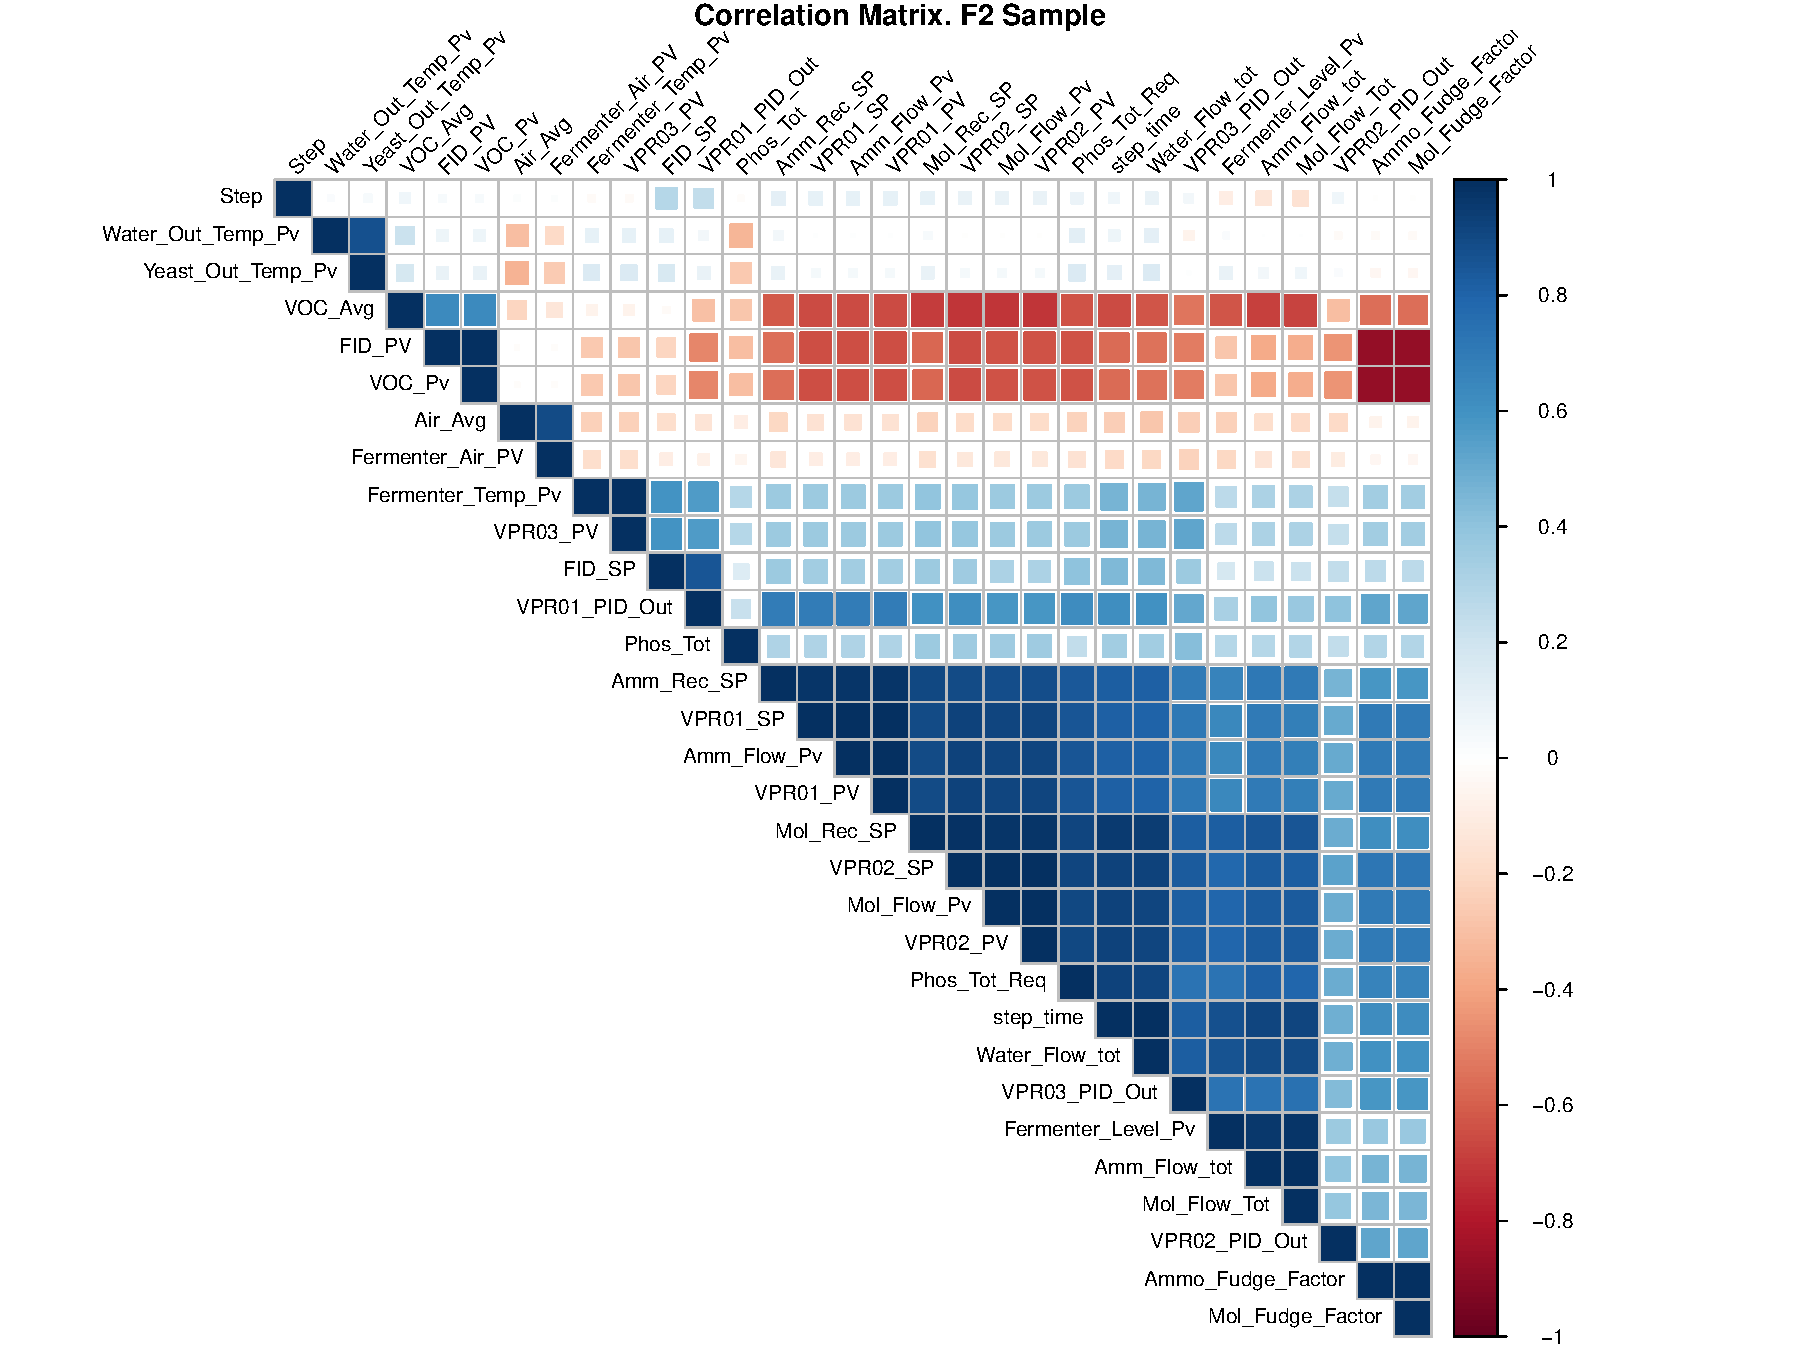
\includegraphics[width=1\textwidth]{plots/f2_correlation.pdf}
    \caption{F2 correlation matrix}
    \label{fig:f2_correlation}
\end{figure}

\begin{figure}[ht]
    \centering
    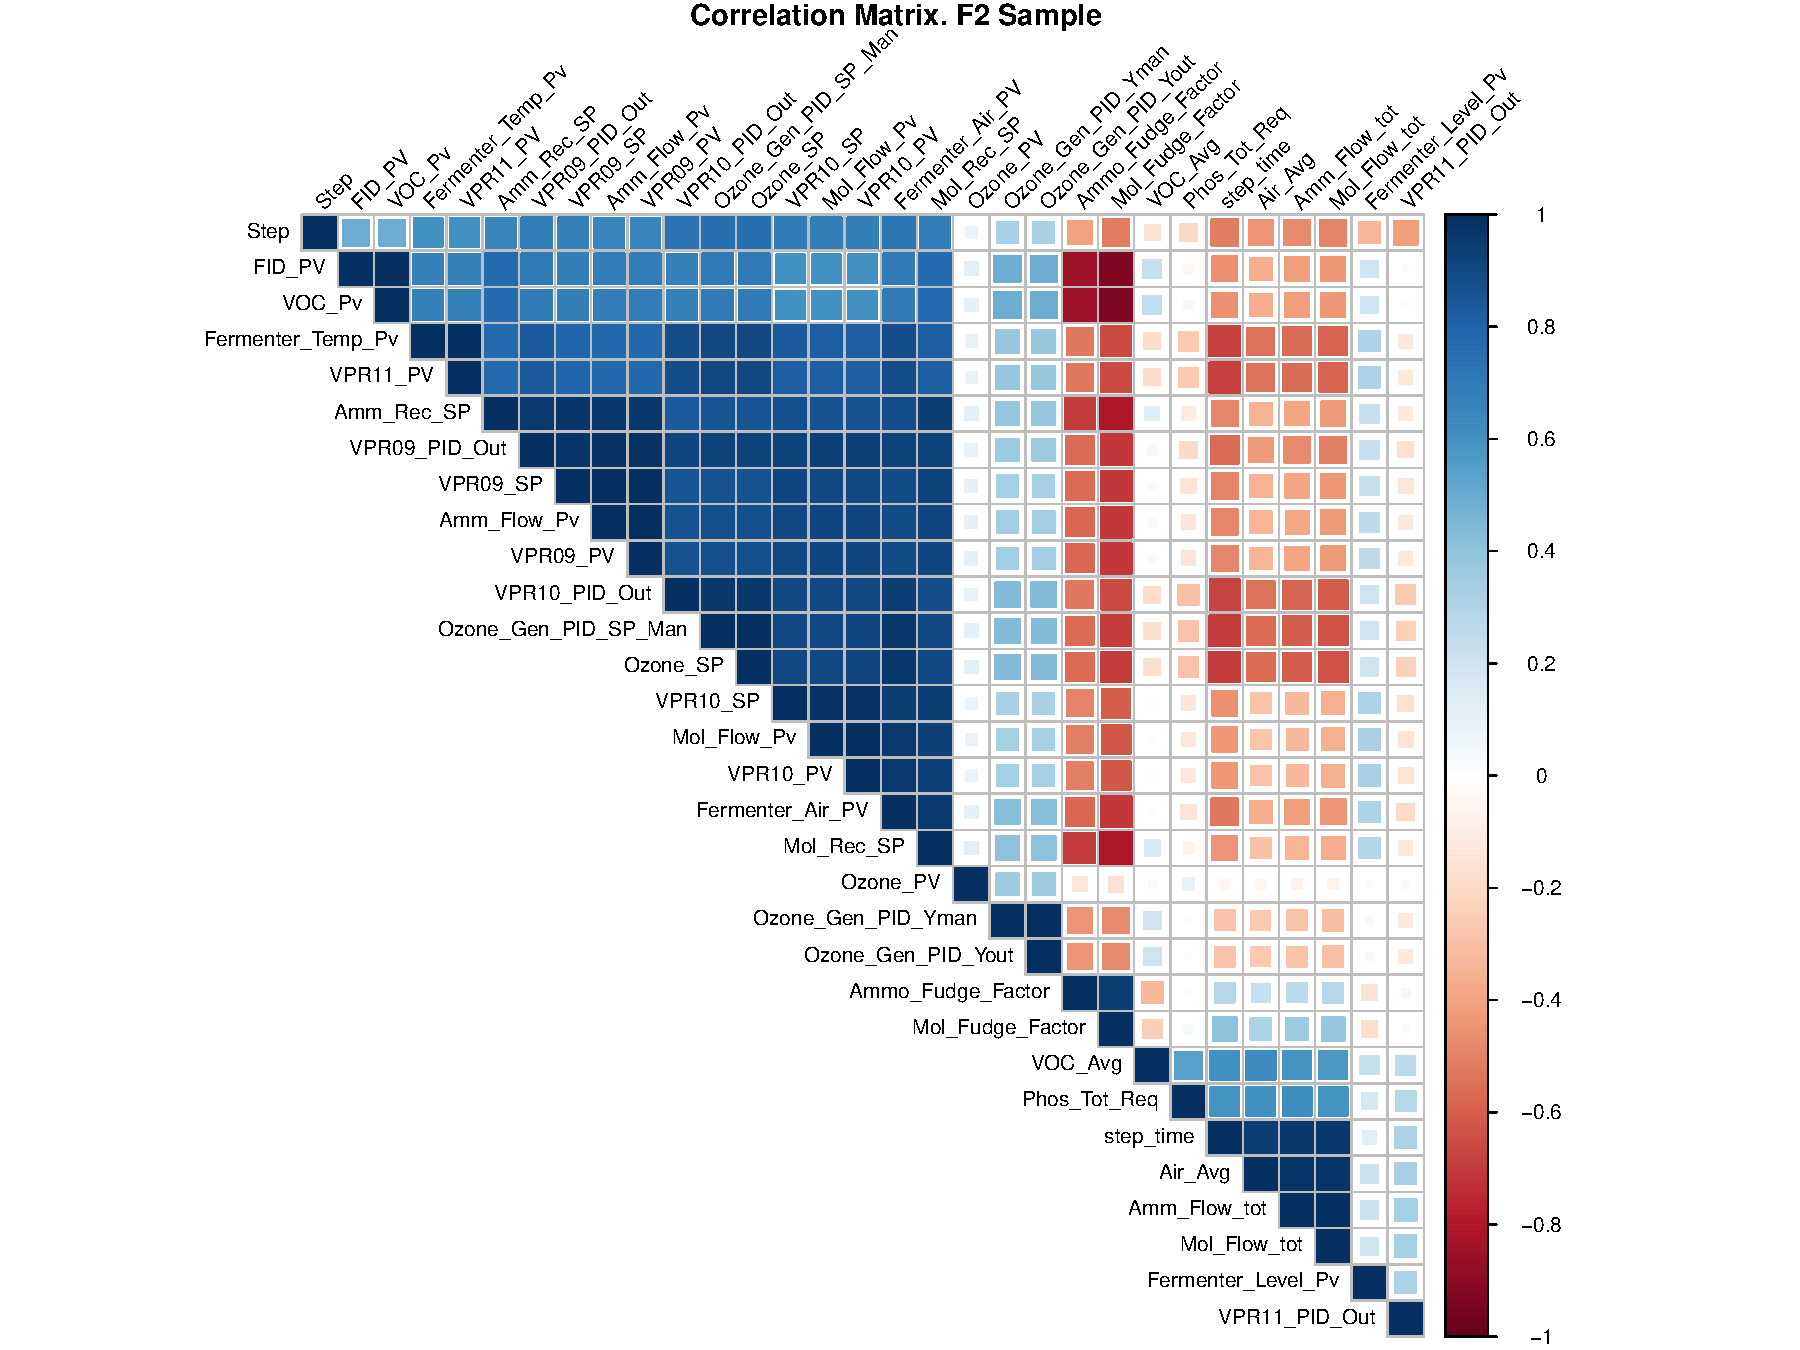
\includegraphics[width=1\textwidth]{plots/f4_correlation.pdf}
    \caption{F4 correlation matrix}
    \label{fig:f4_correlation}
\end{figure}

\begin{figure}[ht]
    \centering
    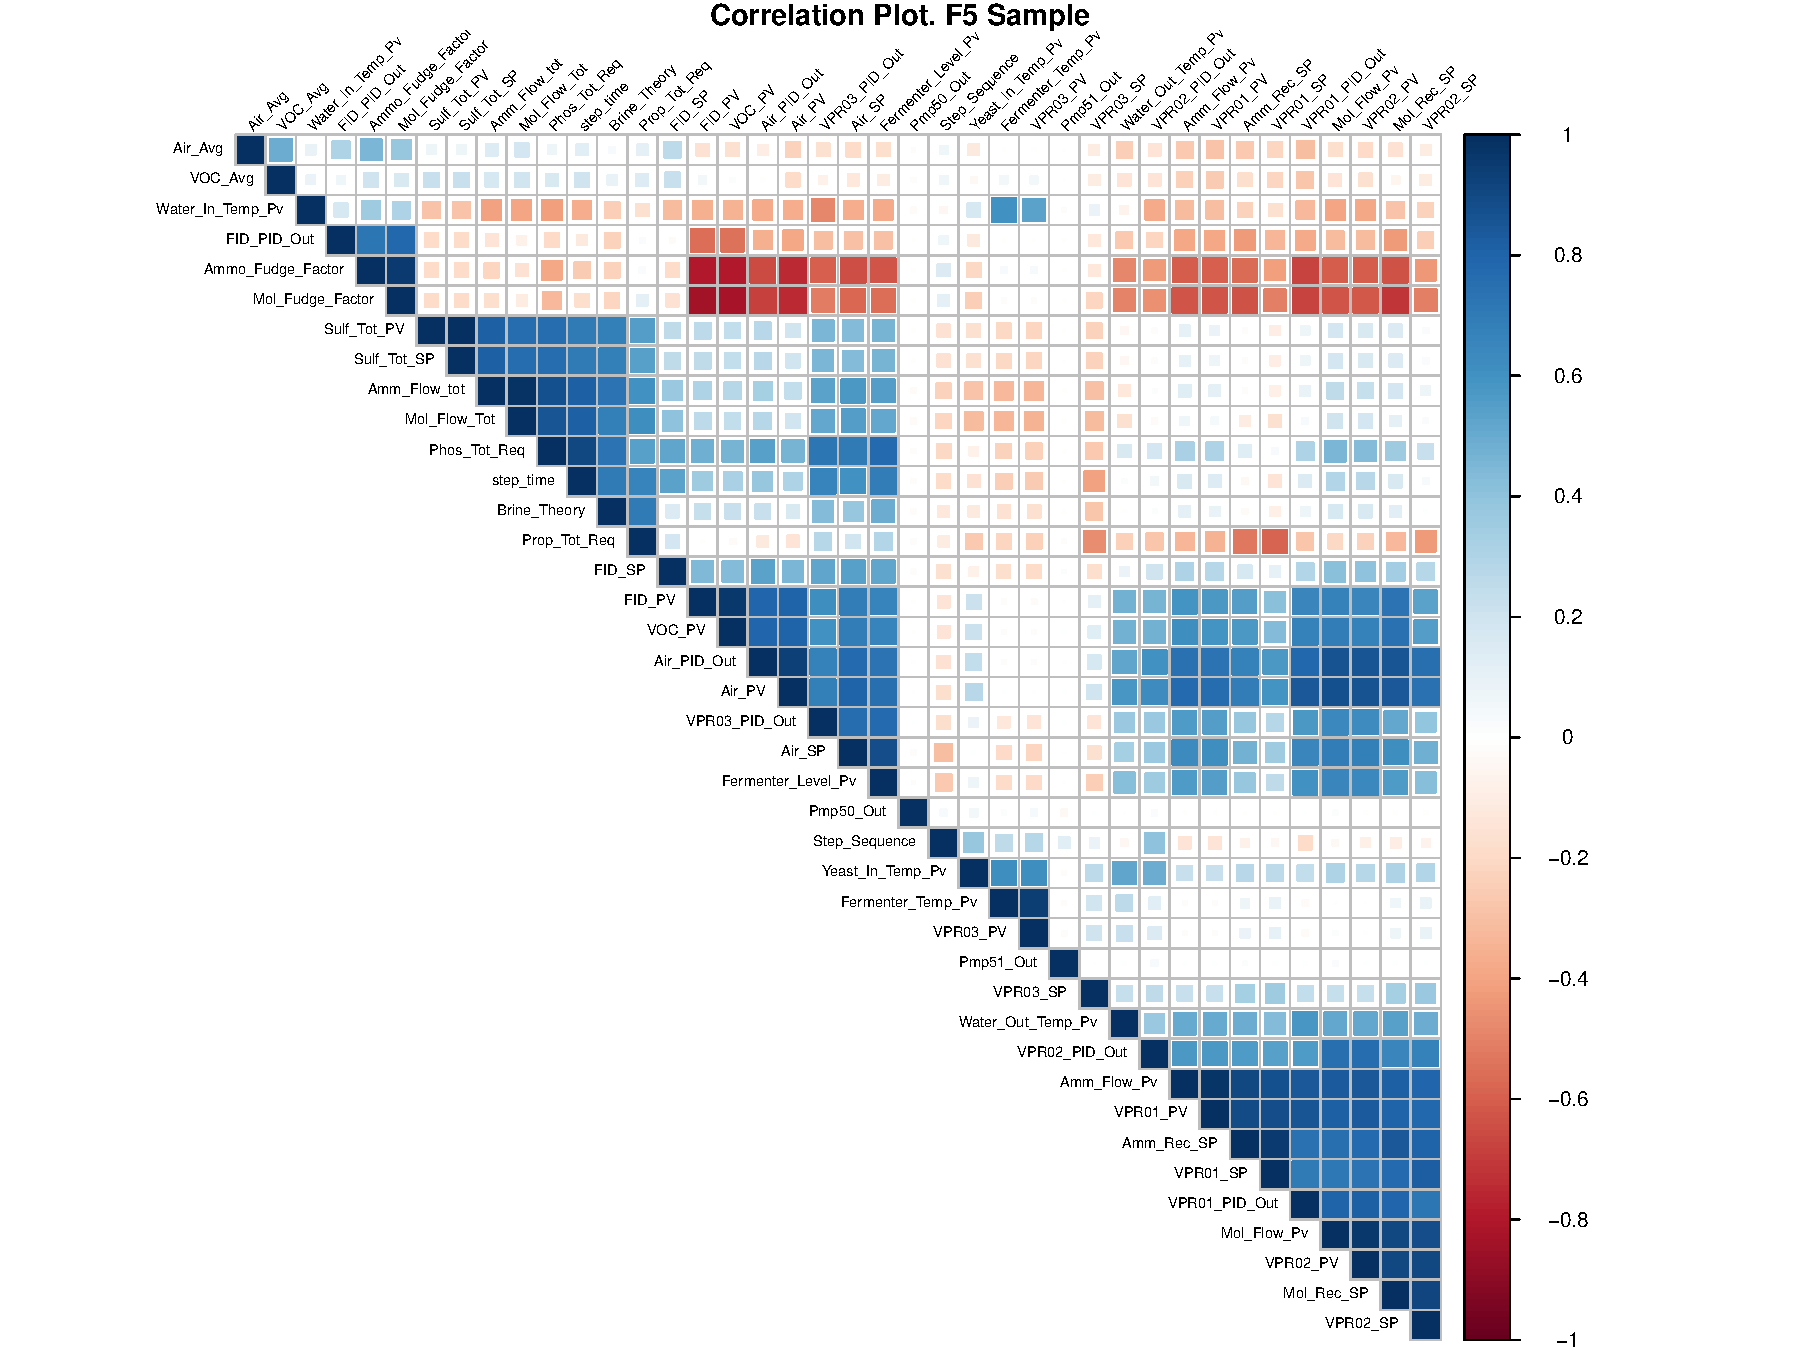
\includegraphics[width=1\textwidth]{plots/f5_sample_correlation.pdf}
    \caption{F5 correlation matrix}
    \label{fig:f5_correlation}
\end{figure}




\end{document}
